\chapter{Basic Statistics in Spreadsheets}

When you completed the problems in the last section, you probably noticed
how long it took to compute statistics like the mean, the median,
and variance by hand. Luckily, computers were designed to free us from these
sorts of tedious tasks. The most basic tool for automating
calculations is the spreadsheet program.\index{spreadsheet}

There are lots of spreadsheet programs including Microsoft's Excel and
Apple's Numbers. Any spreadsheet program will work; they are all very
similar. The instructions and screenshots here will be from Google
Sheets -- a free spreadsheet program you use through your web browser.

\section{Your First Spreadsheet}

In whatever spreadsheet program you are using, create a new spreadsheet document.

A spreadsheet is essentially a grid of cells. In each cell you can put data (like numbers or text) and formulas.

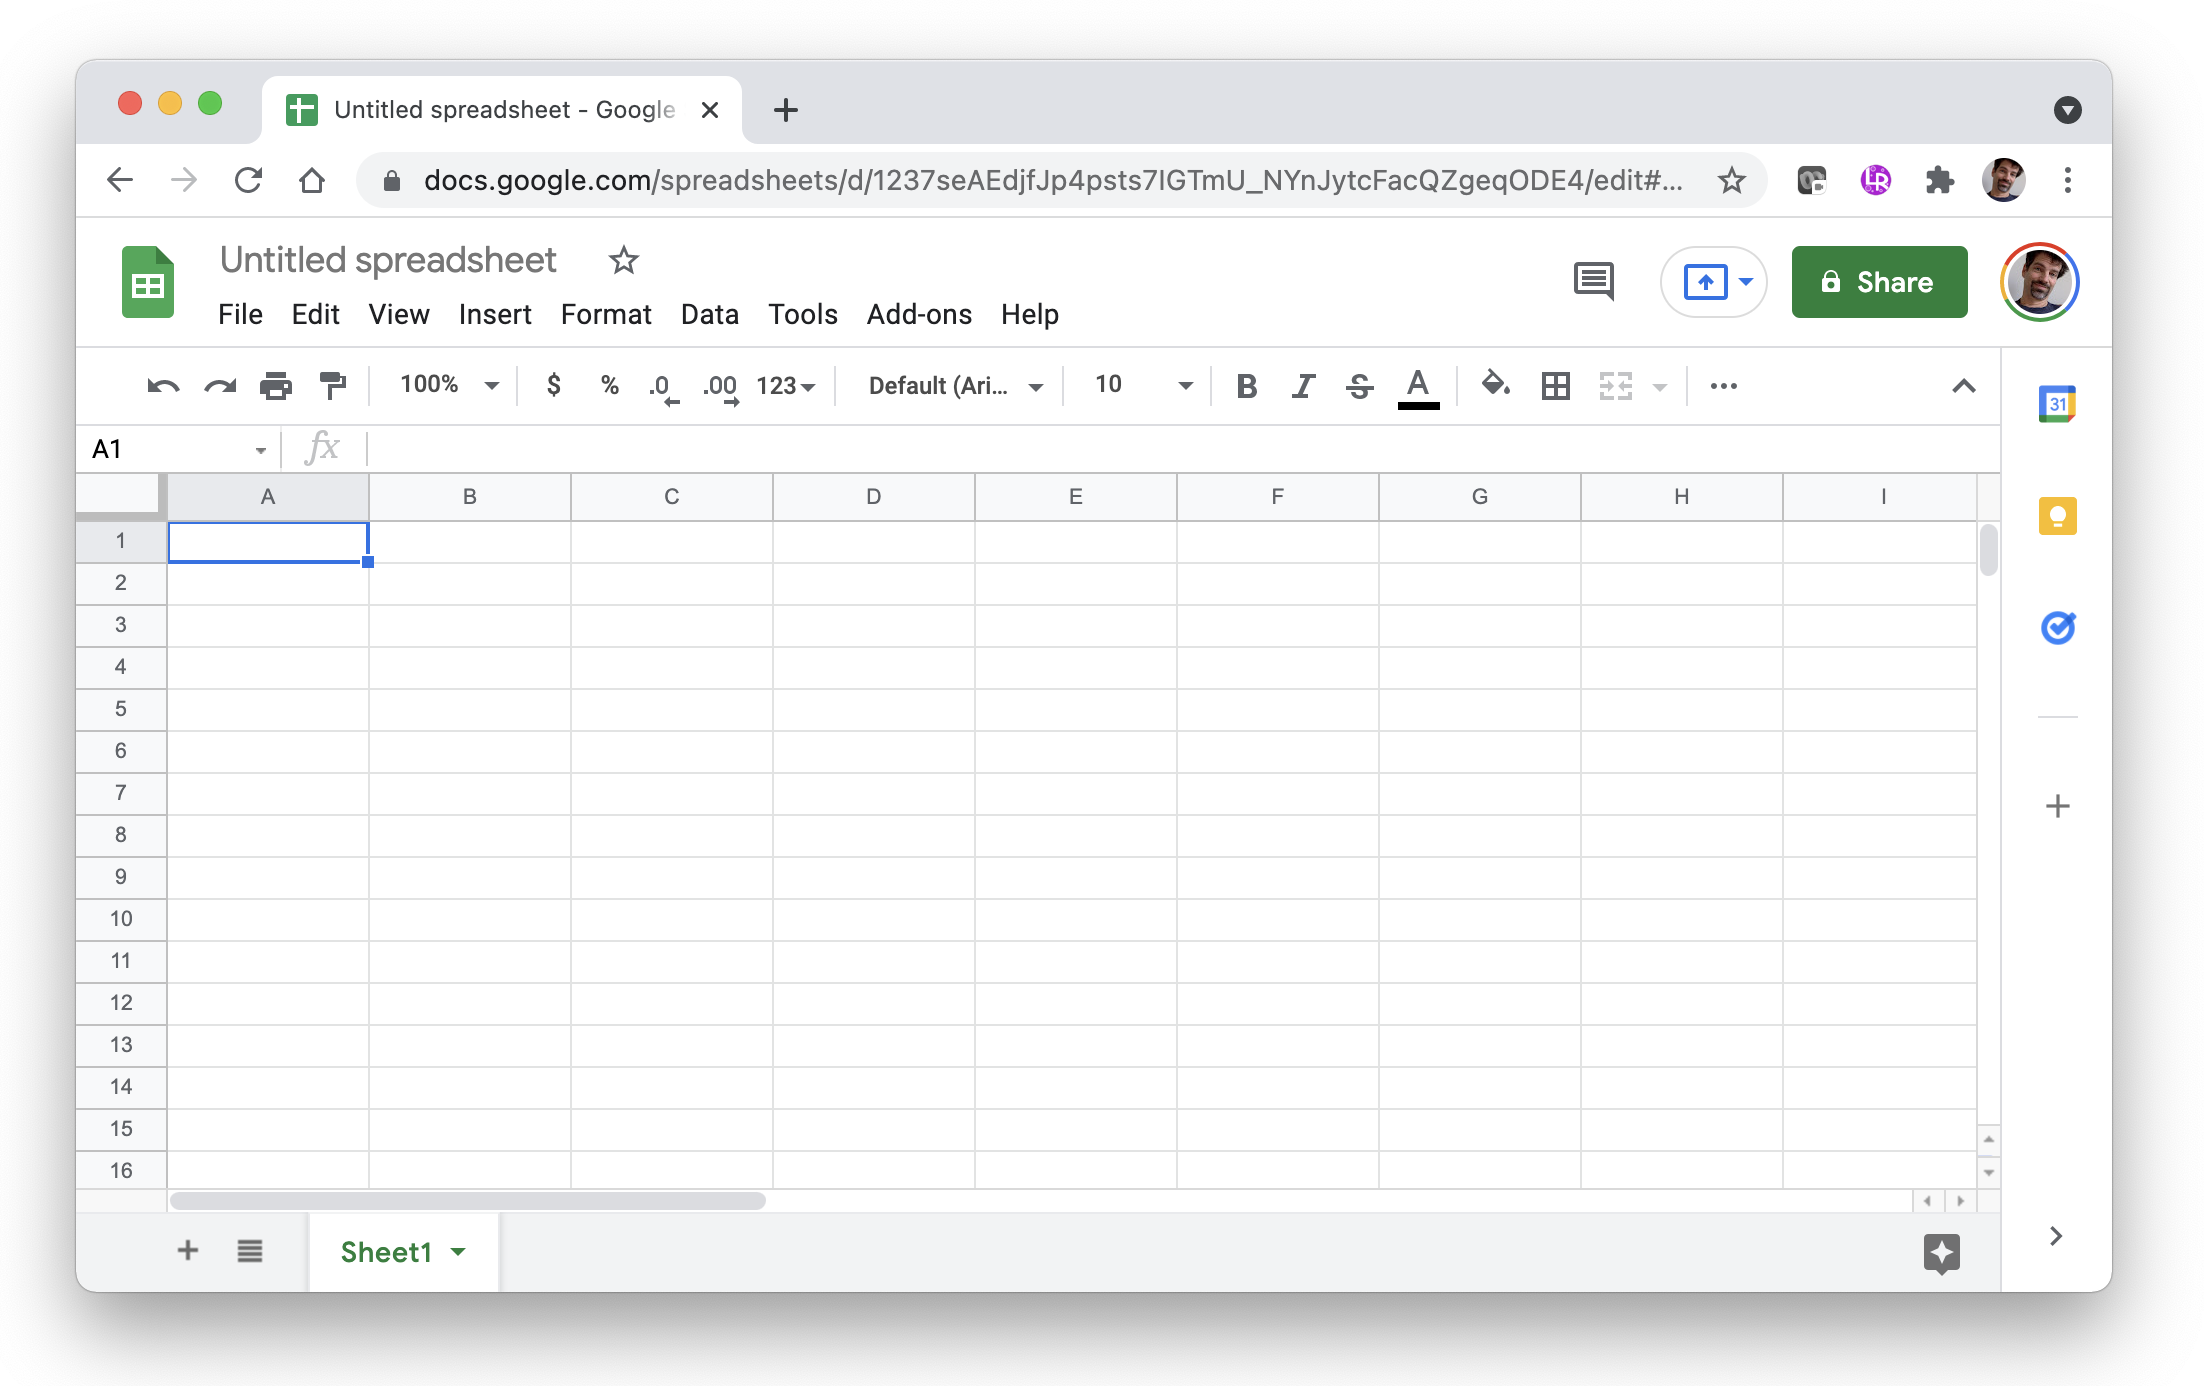
\includegraphics[width=0.6\textwidth]{BlankSheet.png}

Let's put some labels in the column:
\begin{itemize}
\item Select the first cell (A1) and type ``A number''.
\item Select the cell below it (A2) and type ``Another number''.
\item Select the cell below that one (A3) and type ``Their product''.
\item In the next column, type the number 5 in B1 and 7 in B2.
\end{itemize}

It should look like this:

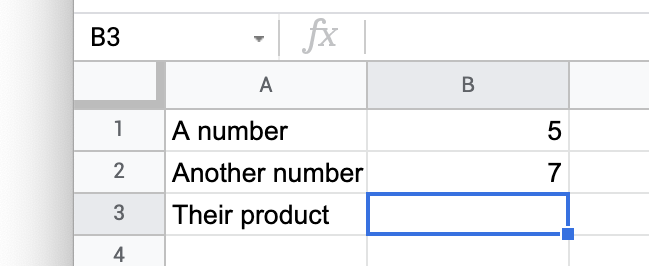
\includegraphics[width=0.5\textwidth]{NoFormulas.png}

Now put a formula in cell B3. Select B3, and type ``= B1 + B2''. The spreadsheet knows this is a formula because it starts with `=`. It will look like this as you type:\index{Spreadsheet!Entering formula}

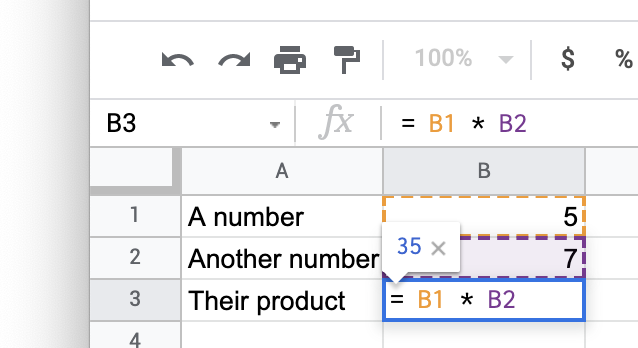
\includegraphics[width=0.5\textwidth]{TypingFirstFormula.png}

When you press Return or Tab, the spreadsheet will remember the formula, but display its value:

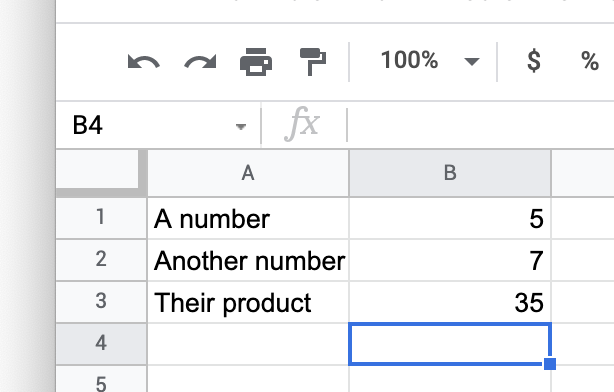
\includegraphics[width=0.5\textwidth]{FirstCalc.png}

If you change the values of cell B1 or B2, the cell B3 will automatically be recalculated. Try it.

\section{Formatting}

Every spreadsheet lets you change the formatting of your columns and cells. They are all a little different, so play with your spreadsheet a little now. Try to do the following:
\begin{itemize}
\item Set the background of the first column to light gray.
\item Right-justify the text in the first column.
\item Make the text in the first column bold.
\item Make the numbers in the second column have one digit after the decimal point.
\end{itemize}

It should look something like this:

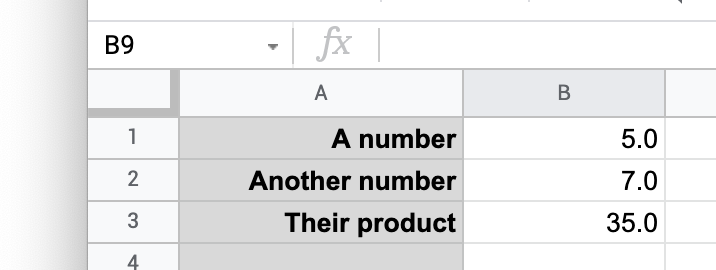
\includegraphics[width=0.6\textwidth]{FirstFormatting.png}

That's a spreadsheet. You have a grid of cells. Each cell can hold a
value or a formula that uses values from other cells. The cells with
formulas automatically update as you edit the values in the other
cells.

\section{Comma-Separated Values}

A lot of data is exchanged in a file format called
\textit{Comma-Separated Values} or just CSV. Each CSV file holds one
table of data. It is a text file, and each line of text corresponds to
one row of data in the table. The data in each column is separated by
a comma. The first line of a CSV is usually the names of the
columns. A CSV might look like this:

\begin{Verbatim}
studentID,firstName,lastName,height,weight
1,Marvin,Sumner,260,45.3
2,Lucy,Harris,242,42.2
3,James,Boyd,261,44.2
\end{Verbatim}

In your digital resources for this module, you should have a file
called \path{1000cars.csv}. It is a CSV with only one column called
``speed''. The first few lines look like this:

\begin{Verbatim}
speed
33.8000
29.9920
34.8699
27.9936
\end{Verbatim}

There is a title line and 1000 data lines.

Import this CSV into your spreadsheet program. In Google Sheets, it looks like this:

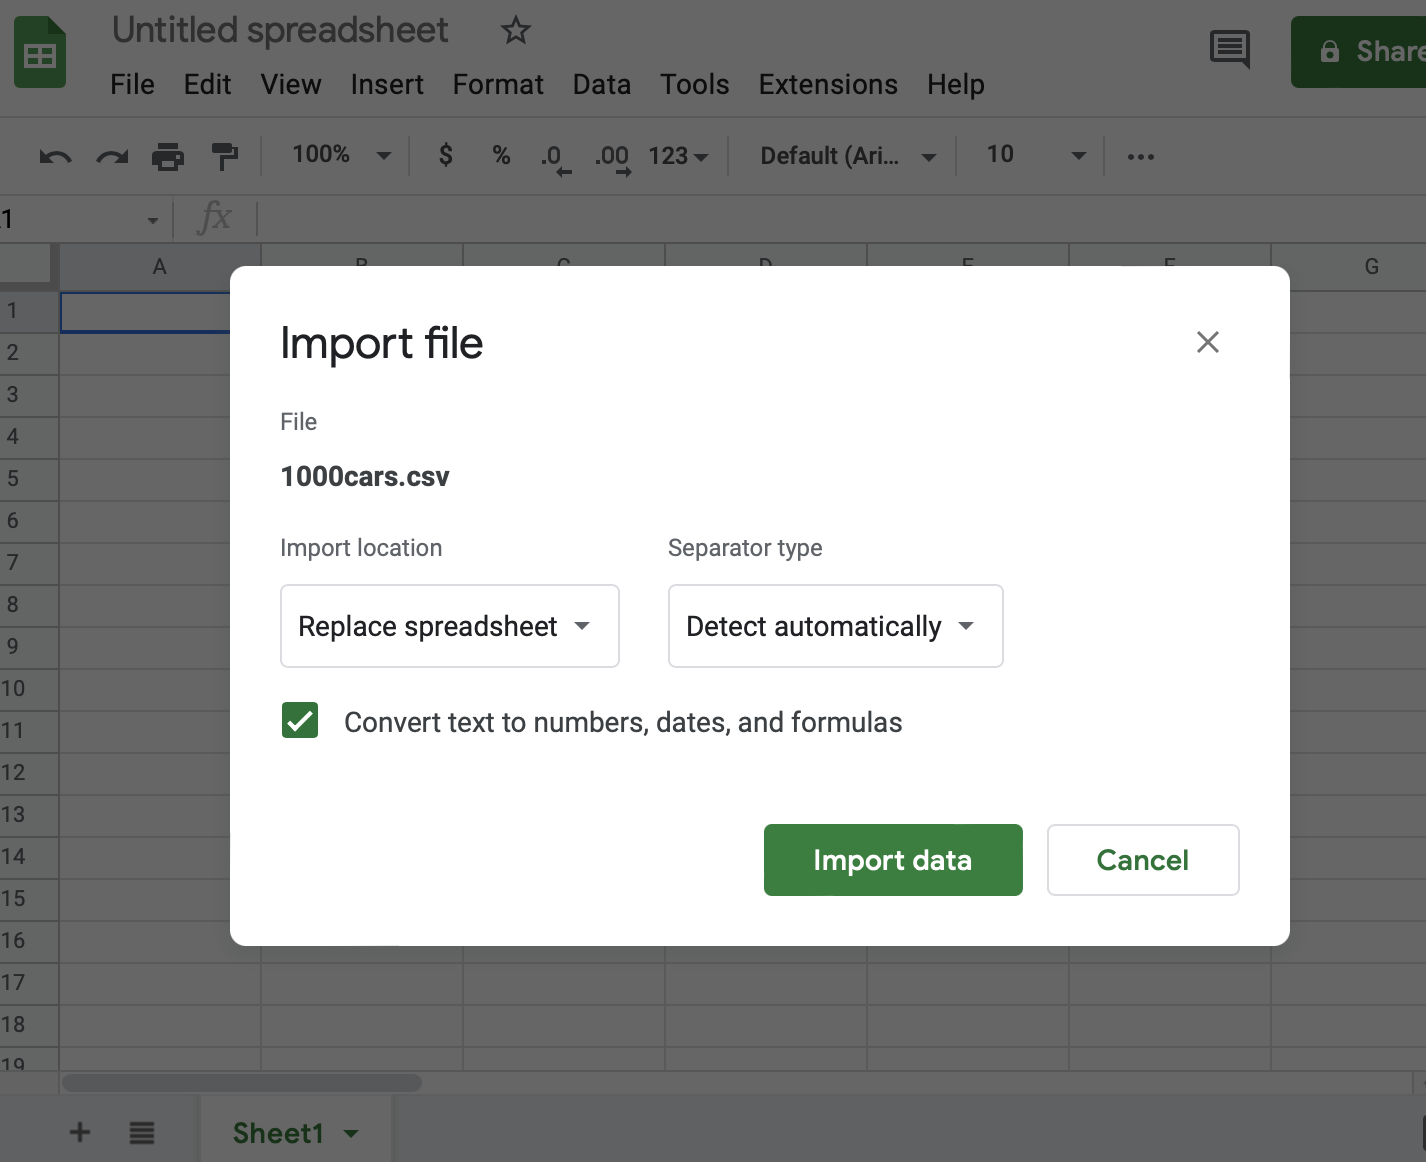
\includegraphics[width=0.5\textwidth]{ImportingCSV.png}

You should see a long, long column of data appear. (Mine goes from cell A2 through A1001.)

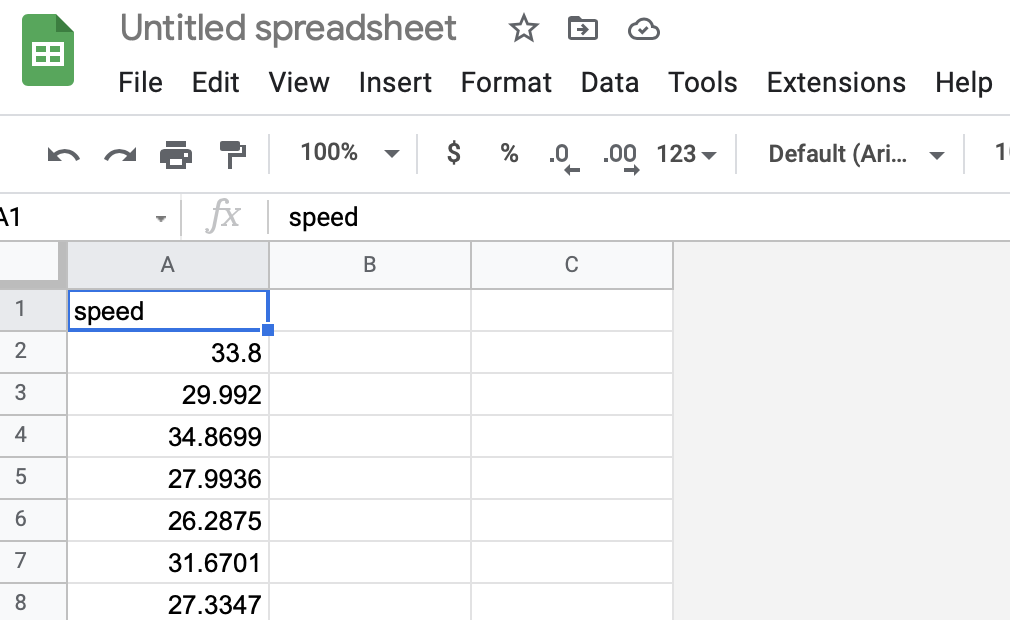
\includegraphics[width=0.5\textwidth]{ImportedCSV.png}

\section{Statistics in Spreadsheets}

Let's take the mean of all 1000 numbers.  In cell B2, type in a label:
``Mean''. (Feel free to format your labels as you wish. Bolding is recommended.)

In cell C2, enter the formula ``=AVERAGE(A2:A1001)''. When
you press return, the cell will show the mean: 31.70441, if done correctly.

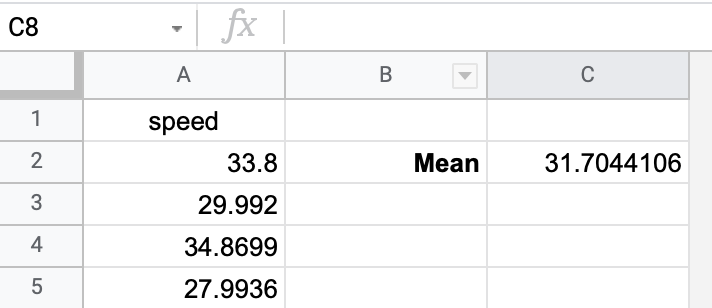
\includegraphics[width=0.4\textwidth]{Spread_mean.png}

Notice that by specifying that the function \pyfunction{AVERAGE} was to
be performed on a range of cells: cells A2 through A1001.

Do the calculations for variance, standard deviation, and median.

\begin{itemize}
\item The function for variance is \pyfunction{VAR}.
\item The function for standard deviation is \pyfunction{STDEV}.
\item The function for median is \pyfunction{MEDIAN}.
\end{itemize}

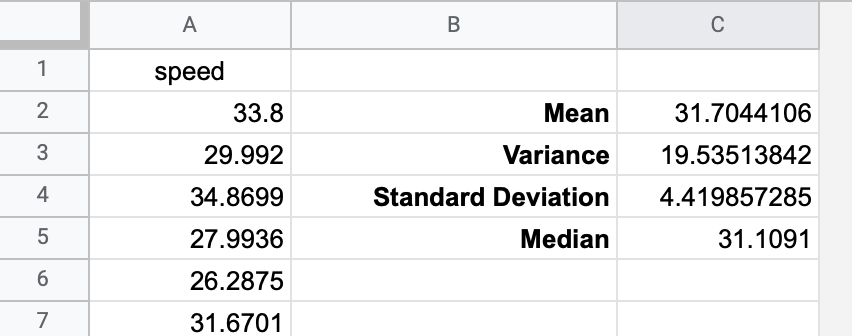
\includegraphics[width=0.4\textwidth]{var_stdev_median.png}

\section{Histogram}

Most spreadsheets have the ability to create a histogram. In Google
Sheets, you select the entire range A2:A1001 by selecting the first
cell and then shift-clicking the last. Then you choose
Insert$\rightarrow$Chart. In the inspector, change the type of the
chart to a histogram. This will get you a basic histogram.
% Add: Define histogram or give example, defined in basic statistics, must come previous

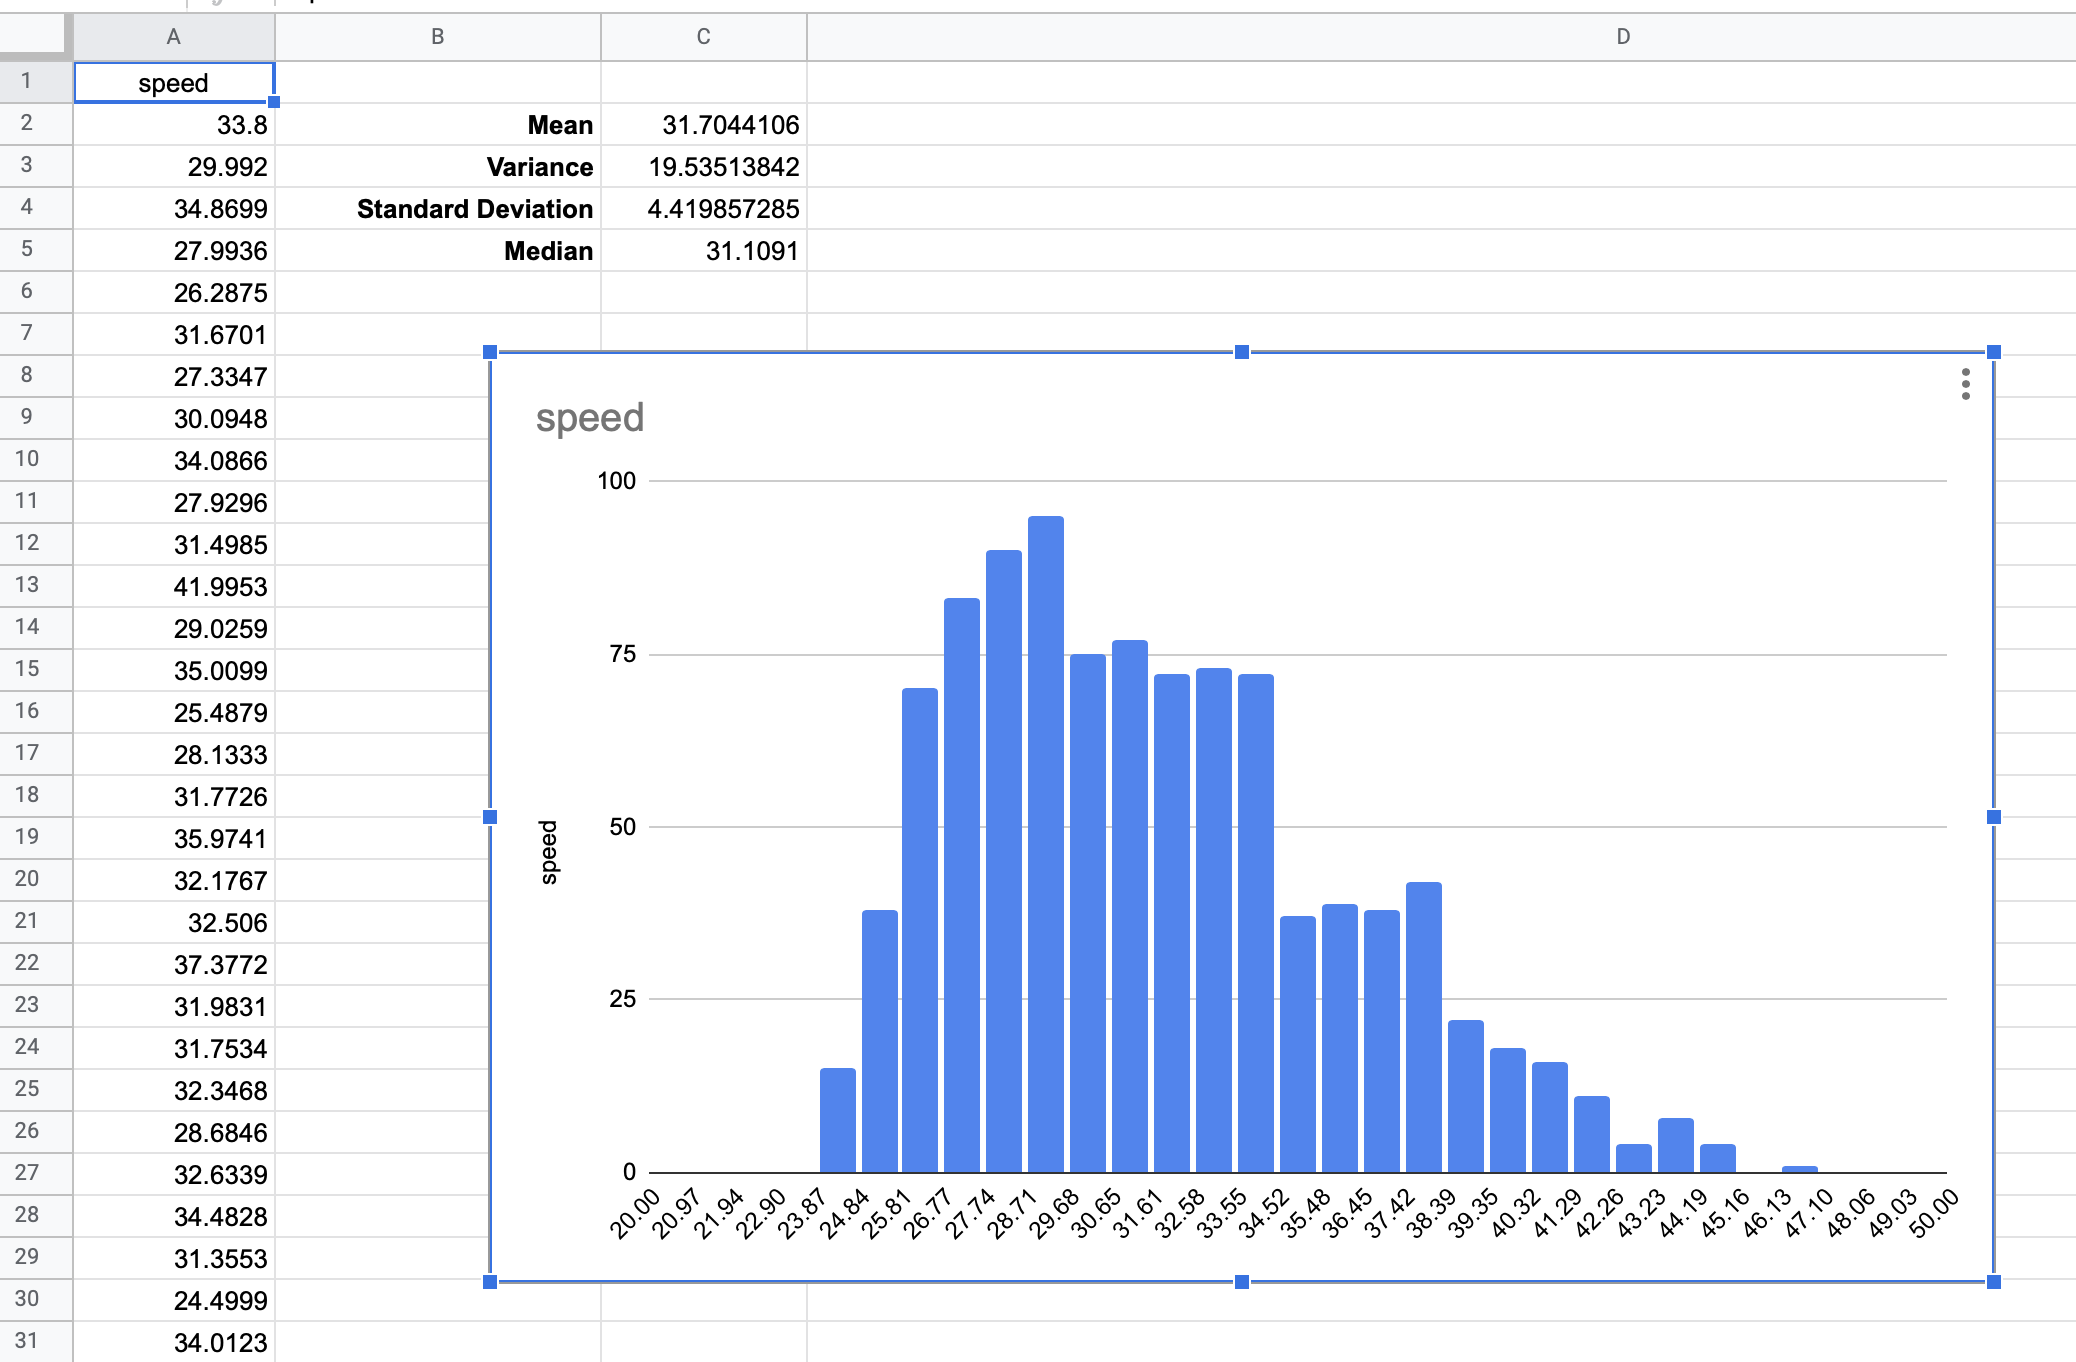
\includegraphics[width=0.7\textwidth]{default_histogram.png}

Play with the formatting to see how unique you can make data. Here is an example:

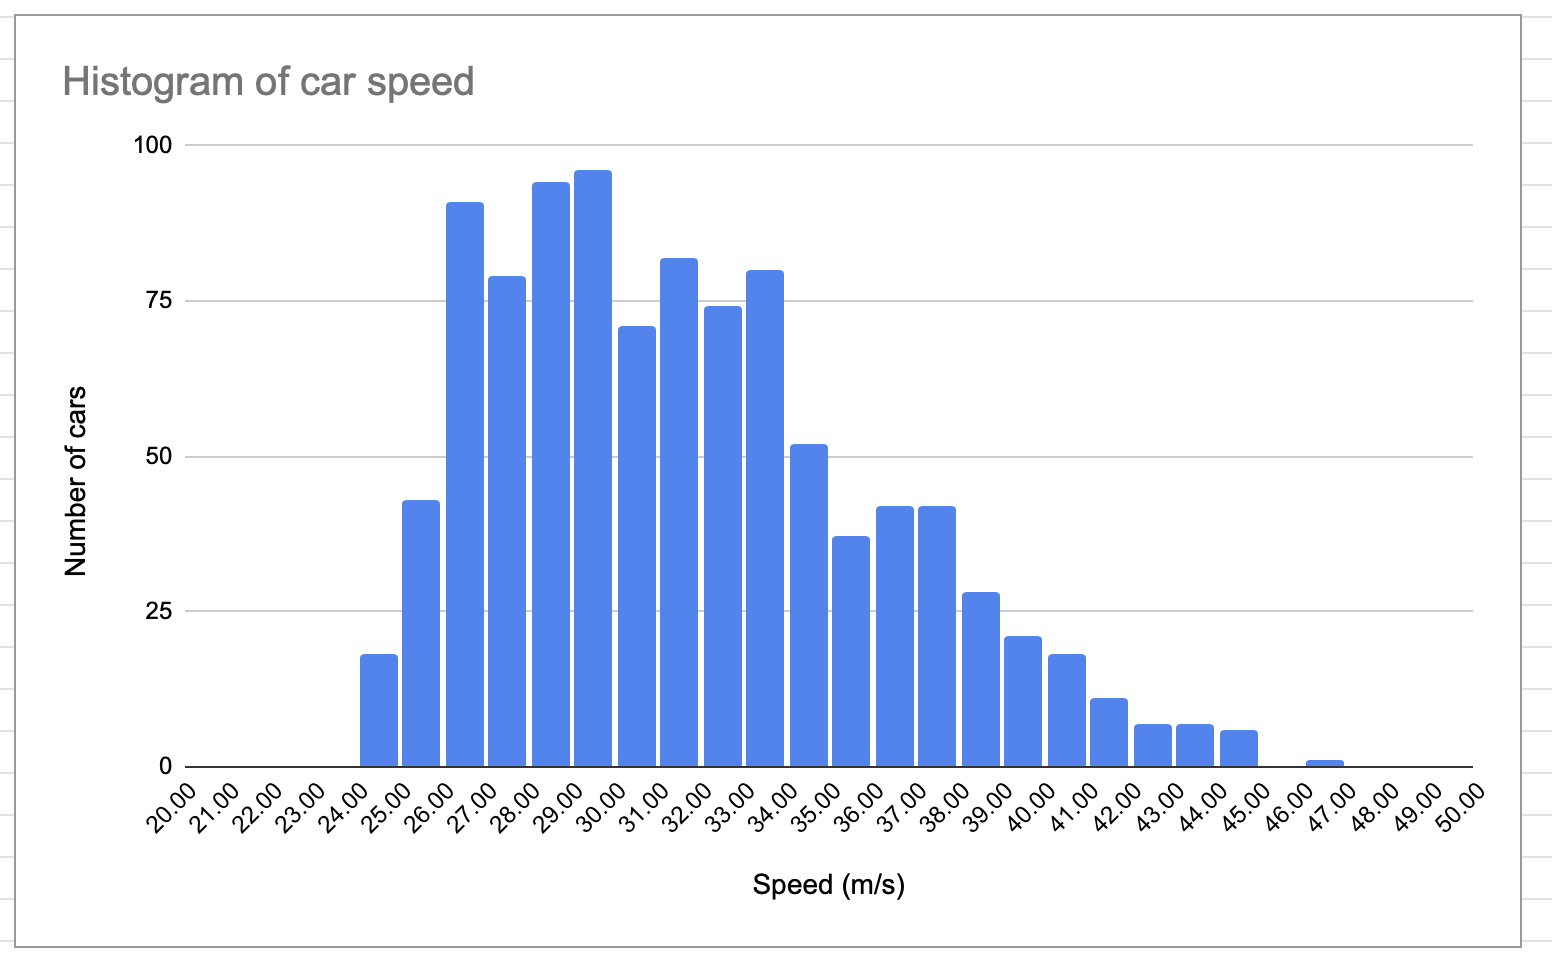
\includegraphics[width=0.8\textwidth]{final_histogram.png}

\begin{Exercise}[title={RMS}, label=rms_spreadsheet]

  In your spreadsheet, calculate the quadratic mean (the root-mean-squared) of the speeds.

  You will need the following three functions:
  \begin{itemize}
  \item \pyfunction{SUMSQ} returns the sum of the squares of a range of cells.
  \item \pyfunction{COUNT} returns the number of cells in a range that contains numbers.
  \item \pyfunction{SQRT} returns the square root of a number.
  \end{itemize}


\end{Exercise}
\begin{Answer}[ref=rms_spreadsheet]

The formula for the RMS is ``=SQRT(SUMSQ(A2:A1001)/COUNT(A2:A1001))''.
% KA: https://www.khanacademy.org/computing/ap-computer-science-principles/data-analysis-101/data-tools/a/learning-from-data-sets

\end{Answer}

